\subsubsection{BI-LSTM Results}

After implementing the architecture recommended in \cite{fieri2023offensive} and training it for 200 epochs using Twitter-RoBERTa embeddings, the following results were obtained:

\begin{figure}[H]
    \centering
    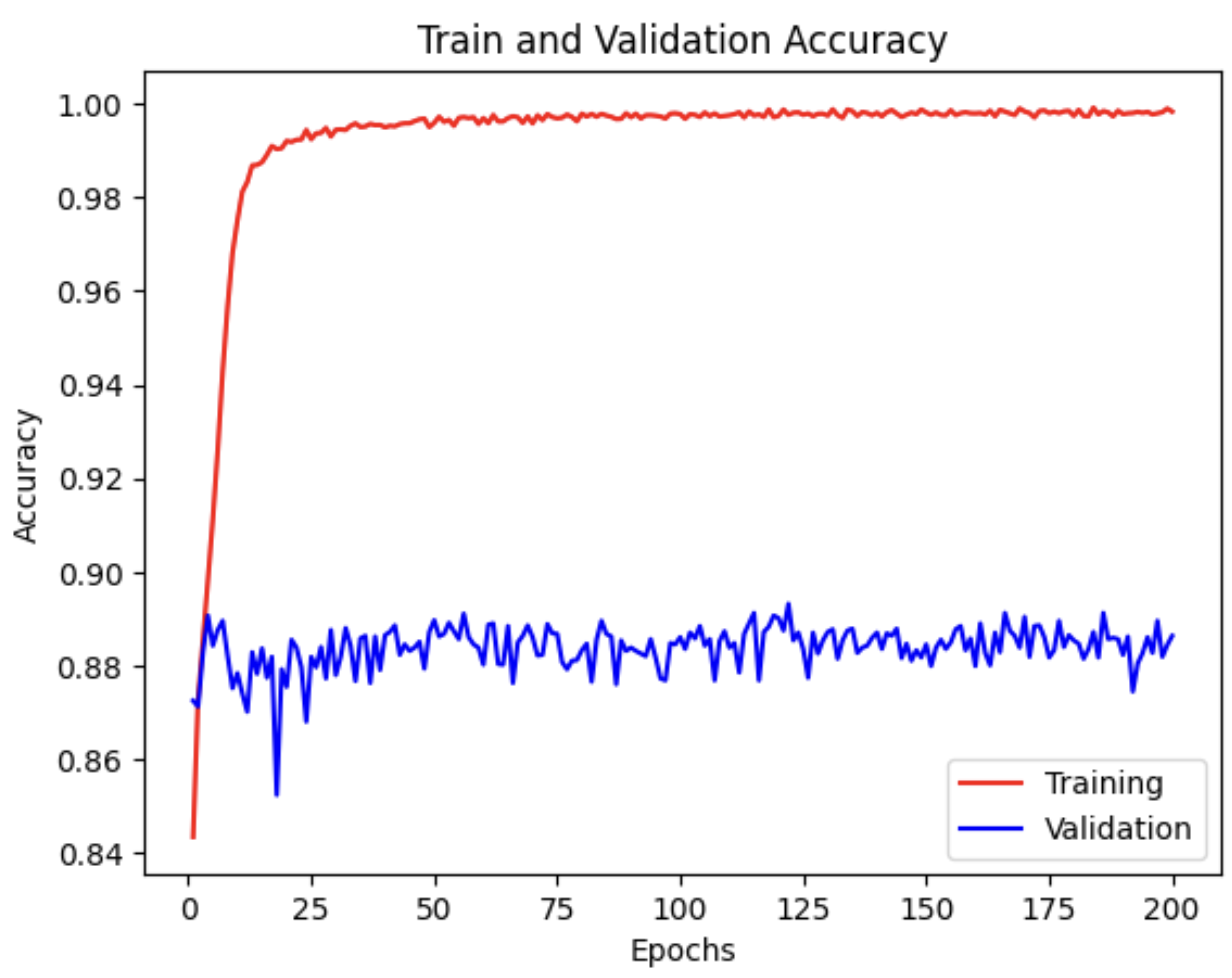
\includegraphics[width=0.45\textwidth]{images/trainingValidationAccurayBI_LSTM.png}
    \caption{Training and Validation Accuracy for BI-LSTM model using Twitter-RoBERTa embeddings}
    \label{fig:accuracy_bilstm}
\end{figure}

\begin{figure}[H]
    \centering
    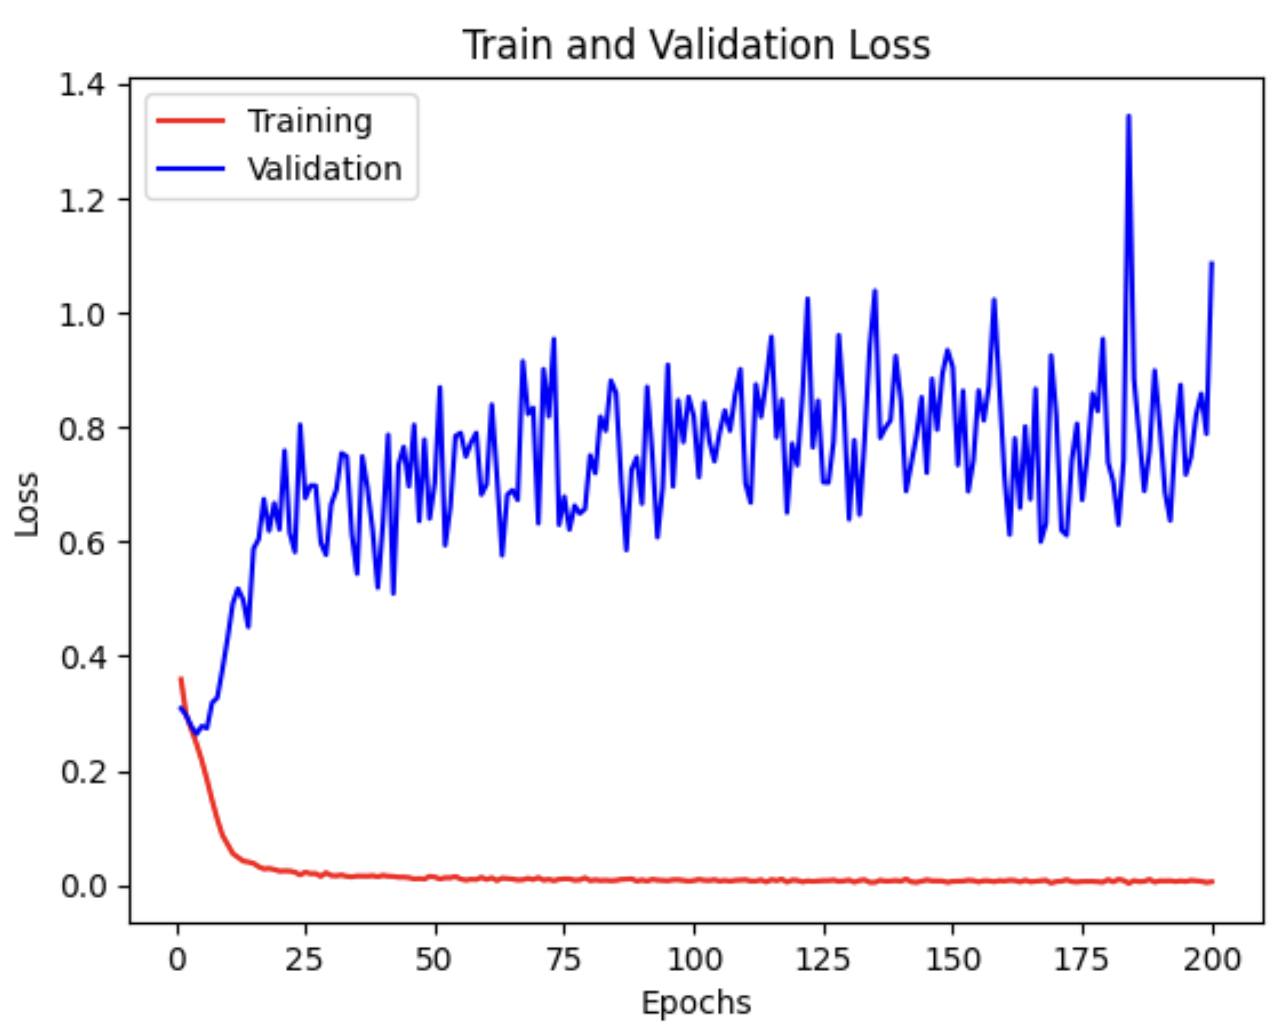
\includegraphics[width=0.45\textwidth]{images/trainingValidationLossBI_LSTM.png}
    \caption{Training and Validation Loss for BI-LSTM model using Twitter-RoBERTa embeddings}
    \label{fig:loss_bilstm}
\end{figure}

As shown in Figures \ref{fig:accuracy_bilstm} and \ref{fig:loss_bilstm}, the BI-LSTM model quickly overfits the training data. The training performance is very high, with a loss approaching 0 and an accuracy near 1. In contrast, the validation set shows worse results, with loss values ranging between 0.5 and 1.4, and accuracy stabilizing around 0.88.

Due to this oscillating behavior, with several performance spikes, a checkpoint was saved using the best validation accuracy. This peak occurred at epoch 122, achieving an accuracy of 0.89321. This represents a significant improvement compared to other results, such as those obtained with XGBoost. However, the score approaches—but does not surpass—the results reported in \cite{fieri2023offensive} and \cite{toktarova2023hate}.

\begin{table}[H]
\centering
\caption{Classification Report BI-LSTM}
\label{tab:classification_report}
\begin{tabular}{lcccc}
\toprule
Class        & Precision & Recall & F1-score & Support \\
\midrule
0            & 0.86      & 0.93   & 0.89     & 3517    \\
1            & 0.92      & 0.86   & 0.89     & 3638    \\
\midrule
Accuracy     &           &        & 0.89     & 7155    \\
Macro Avg    & 0.89      & 0.89   & 0.89     & 7155    \\
Weighted Avg & 0.89      & 0.89   & 0.89     & 7155    \\
\bottomrule
\end{tabular}
\end{table}

In Table~\ref{tab:classification_report}, the generated classification report is shown, reflecting the same problem observed with XGBoost: many examples are predicted as "non-toxic." This is particularly evident in the reduced precision for the negative class and the lowered recall for the positive class. Nevertheless, there is a clear improvement across all metrics, approaching 90\%.

\begin{figure}[H]
    \centering
    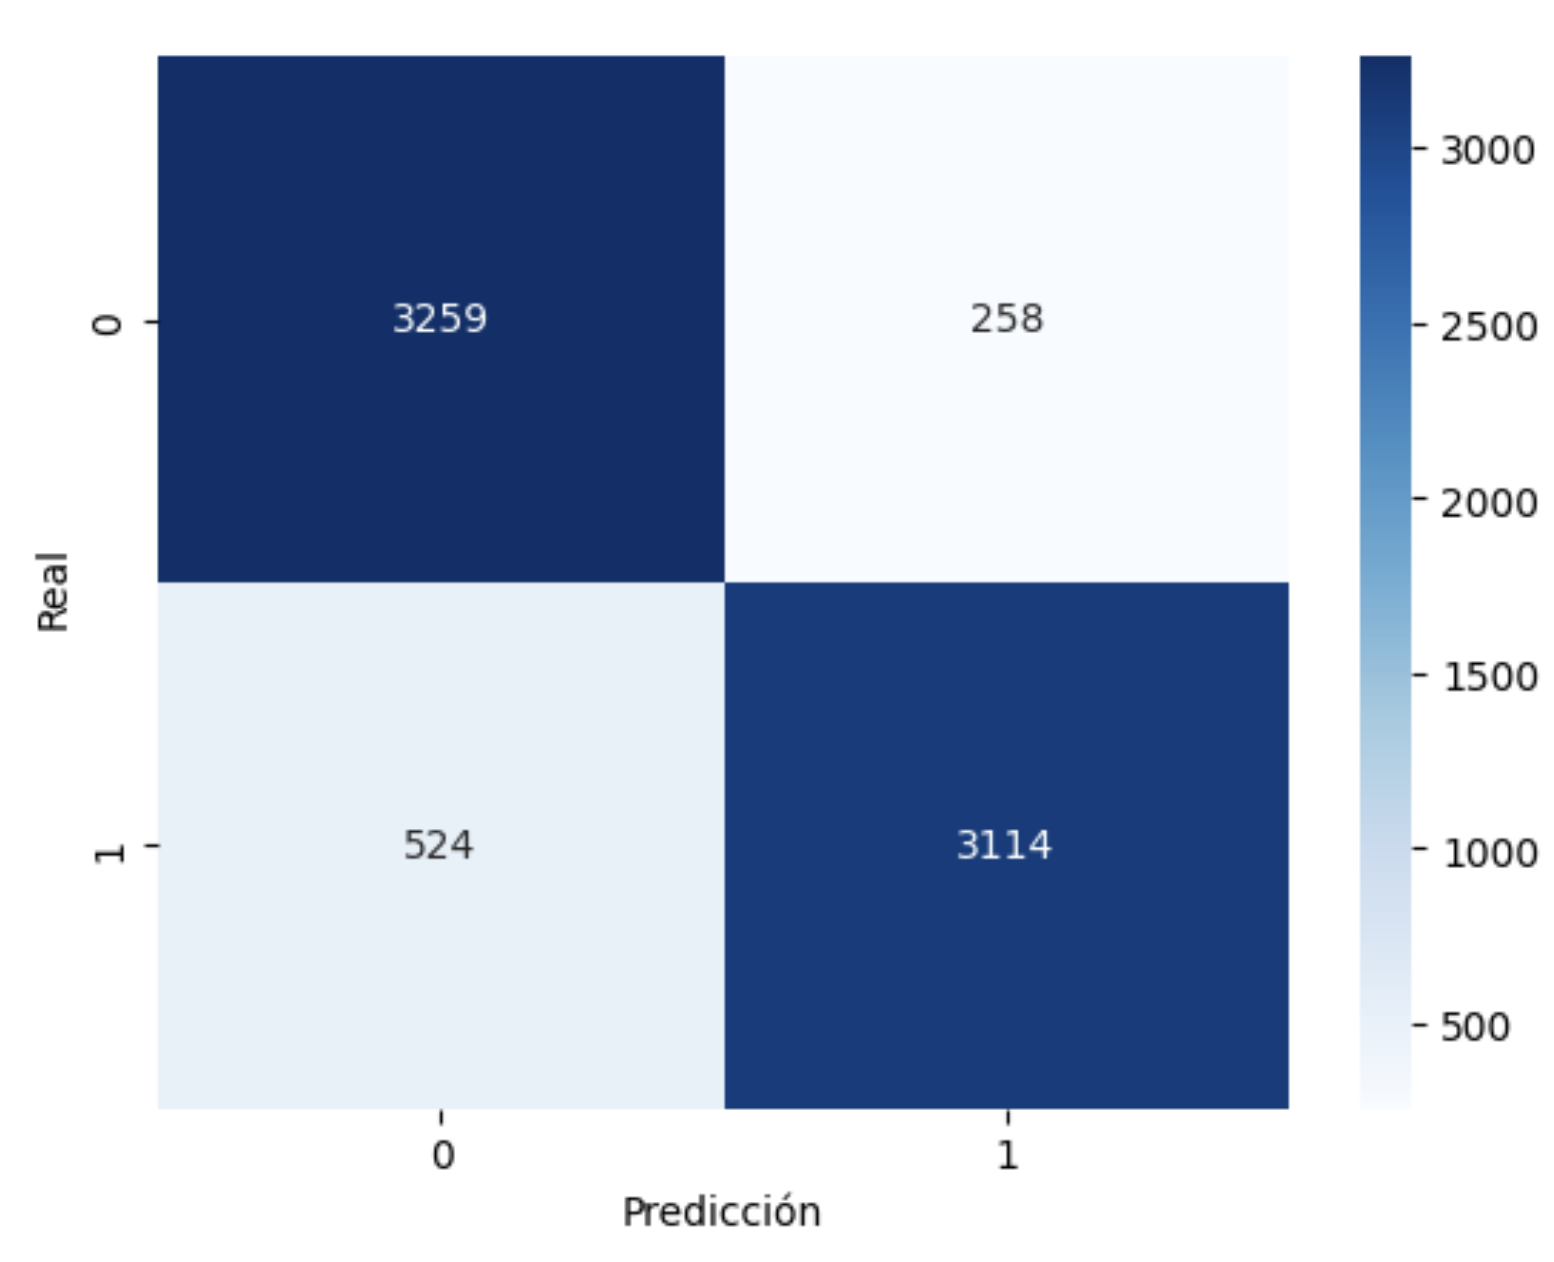
\includegraphics[width=0.45\textwidth]{images/confusion_matrix_bilstm.png}
    \caption{Confusion matrix of the BI-LSTM model}
    \label{fig:confusion_matrix_bilstm}
\end{figure}

In Figure \ref{fig:confusion_matrix_bilstm}, the confusion matrix is shown, where predictions are more focused on true positives and true negatives, with a higher proportion compared to other tested models.